\chapter{Network Analysis}

\newthought{Network analysis can tell us a lot about the most imporant elements of the graph and how well-connected each element is.} A common way is to count the number of connections, shortest paths to neighbors, and shapes that the network takes (i.e. number of triangles).

Some common measures include:
\begin{itemize}
    \item \emph{average degree}, which corresponds to the average number of edges per node. For lastfm, this would mean the average number of artists with whom the genre tag is shared. The higher the number, the more densely connected the network is. A similar measure is graph density, which corresponds to the ratio between number of edges and all possible number of edges.
    \begin{marginfigure}
        \centering
        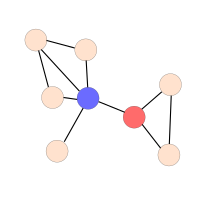
\includegraphics[scale=0.3]{graph.png}
        \caption{The average degree of the above graph is 2.5 (The number of edges for each node divided by the number of nodes.). The degree of the blue node is 5, while the degree for the red node is 3. The degree centrality for the blue node is 0.5 (half of all edges are connected to it!), while for the red node it is 0.3.}
    \end{marginfigure}
    \item \emph{degree}, which is the number of edges per node. The higher the number, the better connected the node is. For lastfm, this would mean the artist with the highest degree would be the one that shares the most genre tags with other artists.
    \item \emph{degree centrality}, which is the ratio of nodes that connect to the given node. A high ratio would mean a node that can reach the most other nodes and that the node is very important in graph structure. In the case of lastfm, this would be the artist that represents the most widely used genre (perhaps pop, rock, jazz).
\end{itemize}
    
But enough talk, let us observe this in practice! A widget that computes these statistics is called \widget{Network Analysis}.

\begin{figure*}[h!]
    \centering
    \newcommand{\hierclust}{\includegraphics[scale=0.45]{net-analysis-graph.png}}
    \newcommand{\imageview}{\includegraphics[scale=0.45]{net-analysis-node.png}}
    \infinitewidthbox{
    \stackinset{r}{-0.45\linewidth}{t}{0.0\linewidth}{\imageview}{\hierclust}\hspace{6cm}
    }
\end{figure*}

\newpage

\begin{wrapfigure}{o}{0.8\textwidth}
    \includegraphics[scale=0.6]{workflow.png}
    \label{fig:embedding}
\end{wrapfigure}

Some statistics relate to graph properties, while others relate to node properties. Select the above three measures. Node statistics will be added to the data table, which means we can observe it in \widget{Network Explorer}.

Sending additional node data to Network Explorer enables us to use the computed statistics in a visualization. We can color the nodes and set their size to degree centrality. This will expose the most central nodes - the ones that share the most tags with their neighbors. Unsurprisingly, we find The Rolling Stones and Britney Spears in the bunch.

\vspace{-0.2cm}
\begin{figure*}[h]
  \centering
  \includegraphics[width=\linewidth]{network-explorer.png}%
  \caption{$\;$}
\end{figure*}
\vspace{-0.3cm}
